\chapter{Security under Android}
\label{chap:and-secu}

\section*{Introduction}
As the number of smartphones is in constant raise, concerns about the security of the system appears.
Paradoxically, the users tends to store more and more personal informations on their smartphone and are not aware of the security issues of such devices.
Malwares have been discovered on the official applications store and antivirus softwares for Android are now sold.
Android runs on top of a Linux kernel which is reputed to be virus free.\\

The aim of this chapter is to explain in detail the actual security mechanisms used to protect the users against malicious applications.
Knowing that, a user should be able to reduce his infection risk by adopting simple security principles.
Is also explained the different procedures to install an application on a device with the risks associated.
The forensic aspect to retrieve information from a device without the owner consent have not been analysed here.\\

These clarifications are essentials to understand the limits and possibilities for the developed \emph{DroidWatcher} (see chapter \ref{chap:droidwatcher}) application to be effective.

\section{Permissions}
For an application to run inside the Android operating system and access to critical resources, it should have explicitly been allowed to do so.
For a set of defined tasks, a permission should be enable.
These tasks are, for example, accessing the current location of the user, update the address book, use Internet, write to the SD card...
At the installation of an application, the permissions necessary are mentioned.\\

The permission system is designed to control the usage of internal Android methods and resources.
Without a permission, an application can not access to certain resources or method in the Android system.

\subsection{Technical details}
In appendix \ref{perm-list}, the list of available permissions are mentioned.
These permissions are defined in the configuration file \texttt{AndroidManifest.xml} present in every application.
Without the correct permission, an application throws an exception when the method accessing the forbidden resource is launched.

\begin{lstlisting}[breaklines,caption={Example of permission violation log},label={lst:gpsexception},numbers=none]
E/AndroidRuntime( 1274): FATAL EXCEPTION: main
E/AndroidRuntime( 1274): java.lang.RuntimeException: Unable to start activity ComponentInfo{com.example.gpstest/com.example.gpstest.MainActivity}: java.lang.SecurityException: Provider gps requires ACCESS_FINE_LOCATION permission
...
E/AndroidRuntime( 1274): Caused by: java.lang.SecurityException: Provider gps requires ACCESS_FINE_LOCATION permission
...
\end{lstlisting}

In the listing \ref{lst:gpsexception}, is shown the Android debugger trace of an application requesting the location of the device using the GPS location provider without having requested the \texttt{ACCESS\_FINE\_LOCATION} permission.
If the error is not caught properly, the execution of the application is interrupted and the users receives a notification of the crash of the application.\\

The permission processed is conceived to control the access to an information and not a phone characteristic.
For example, the \texttt{ACCESS\_COARSE\_LOCATION} permission is not limited to the usage of the high level \texttt{LocationManager} methods but is also required for an application to retrieve the surrounding cell towers informations (as these towers have a unique identifier, this lower level information could also be used to locate the user\footnote{This method is used in the DroidWatcher application to estimate the location even when no network connectivity is available}).

\subsection{Weaknesses}

The way the permission system is implemented does not fully prevent malicious behaviours.
The permission description is unclear and can include different purpose.
For example, the permission \texttt{READ\_PHONE\_STATE} has many purpose.
It allows an application to be aware when a phone call is processed or when the device is locked, it also gives information about the phone unique identifier and SIM id.
This permission is often used to suspend services or simply track a device using the unique identifier.
The problem is that, in case of a phone call, it also provide the access to methods allowing to retrieve the caller phone number.
This is an information leakage that could have been avoided.\\

Also, it is unclear when and why an application requires a permission at the installation process.
Many free applications display advertisements to fund their development.
These kind of applications require the permission to access the internet to download the advertisement content.
A malicious gaming application could justify the need for the two permissions \texttt{INTERNET} and \texttt{WRITE\_EXTERNAL\_STORAGE} (access the microSD card of the device) for advertising and score storing. Using these permission, it could upload the full content of the SD card (which may contains personal informations from the other applications) to a server.
Only a deep analysis such as network monitoring can detect malicious behaviour of an application.\\

Finally, if a user disagree with the need of a suspicious permission, it has no other choice than not install the application.
There is no possibility to partially accept the permissions.
Due to this restriction, if they want to use the application, we can assume than most users will accept, whatever the asked permissions are.

\section{Applications installation}

Unlike iOS where the App Store is the only permitted source of applications\footnote{Alternative markets and applications distributions exists on iOS but they require jailbreaking which is not allow by Apple}, the Android operating system propose several way to install an application.

\subsection{Play Store}
By default\footnote{The Play Store is available only on official Android devices approved by Google. The Android operating system is open source which allows the port on many devices but the Android Play Store application is not and compatible to approved devices only.}, the Android Play Store (previously named Android Market before its merging with Google Music) is the only source of application.
Once a Google account associated to the user's phone, it can use the application Google Play Store which list the available applications and install it quickly.
The figure \ref{fig:market} shows an example of the interface of the application.\\

\begin{figure}[h]
  \centering
  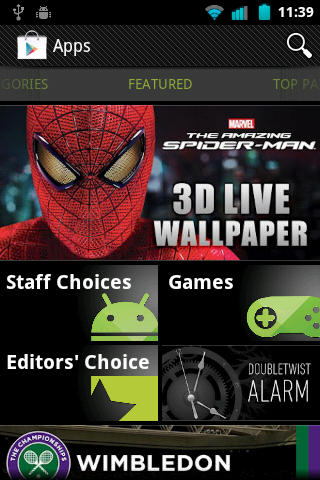
\includegraphics[width=4cm]{images/market1.png}
  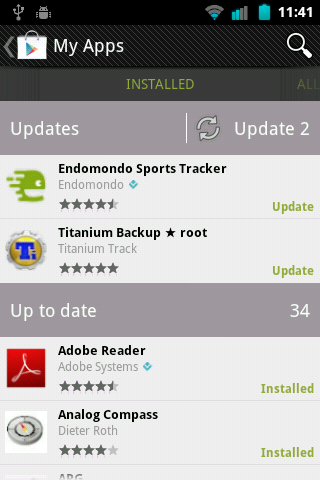
\includegraphics[width=4cm]{images/market2.png}
  \caption{Google Play Store interface}
  \label{fig:market}
\end{figure}

The Android Play Store as several features that can be handy for the average user:
\begin{itemize}
\item warning when an update is available
\item control by Google to avoid malwares
\item user comments and review
\item paid system with Google Checkout
\end{itemize}

Even when distributed by the Play Store, the user should check the asked permission carefully.
This is valid at each update where the permissions can change.
Several cases of malicious applications on the Play Store have been detected in the past (see bellow).
If the approval by Google of each application is a considerable protection it is not perfect and the Play Store should not be considered as a fully safe application distribution medium.\\

On the website \url{https://play.google.com/store}, the content of the Android Play Store is available from a browser.
An important feature of this website is the possibility, once logged with the associated Google account, to select applications to install.
The next time the Android device is connected to the internet, it will automatically download and install the selected application without any user interaction requiered.
A simple notice is displayed on the phone once the application is installed.\\

To distribute an application on the Android Play Store, the registered developer can upload his application on Google Play servers and make it available in a few hours\footnote{Official Distribution Control guidelines \url{https://developer.android.com/distribute/googleplay/about/distribution.html}}.
There is no control before the publication of an application.\\

In the case of an attacker gaining access to the Google account of an Android user, it could remotely install any application.
This would allow the attacker to do almost any kind of actions the device is capable of.
It would be possible to monitor the activity of the user or remotely command the phone.
The developed application \emph{DroidWatcher} is an example of what would be possible with a focus on the geolocalization.

%http://androidforums.com/android-applications/36936-android-permissions-explained-security-tips-avoiding-malware.html

\subsection{Other sources}
By default, installing applications from other source than the Play Store is disallowed.
Changing this setting is proposed when a user is trying to install a software from another source for the first time.

\subsubsection{.apk file}
The \emph{.apk} extension is the convention for installable applications on the Android operating system in the same way as \emph{.deb} or \emph{.rpm} are on Debian and Fedora operating systems.\\

A user trying to open such files on his device launches the installation process in the same way as if he was using the Android Play Store.
The required permissions are displayed and ask for the approval of the user.
The figure \ref{fig:perm-dw} shows the permission screen when a user tries to install the application DroidWatcher.
This is the same screen while using either the Google Play Store or installing an \emph{.apk} file.\\

\begin{figure}[h]
  \centering
  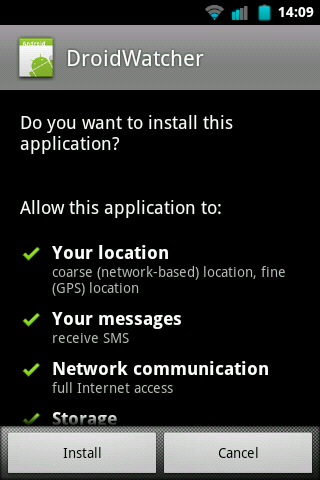
\includegraphics[width=5cm]{images/permissions.png}
  \caption{Permissions requiered to install DroidWatcher}
  \label{fig:perm-dw}
\end{figure}

An apk file is produced after the compilation of a program and is often proposed on small projects or for beta versions.
Also, websites have appear as proposing apk files of non-free applications on the Play Store.
These applications should be considered as are the warrez websites on the Windows operating system: highly risky in term of malwares propagation, these applications could have been manipulated to inject malicious code.\\

Once an application is installed on the system, the apk file is stored on the system.

\subsubsection{Alternative marketplace}
In the same way as the Android Play Store, it exists several alternative market places.
Alternative market places are a way to download apk files from a centralized interface.
It is seen as an alternative to the Google Play Store with the advantages of a centralised distribution medium (paid system, users reviews, moderation...).\\

As for the Play Store, alternative market places are as secured as the control of their owners over the applications acceptance process.
The \emph{Amazon AppStore}\footnote{Available in the US only at \url{http://www.amazon.com/appstore}} developed by Amazon.com Inc. has an approval process to publish applications\footnote{Approval Process and Content Guidelines \url{https://developer.amazon.com/help/faq.html#Approval}}.
%\emph{jesaispluslenom} on the other hand as a fewer control which leads to finding more malicious applications or pirated versions of non-free applications available on the Play Store.

\subsubsection{Debug mode}
If the debug mode of an android device is turned on (done in the configuration settings of the device), interaction between a computer and the device is possible.
Using the official Android Debug Bridge toolkit\footnote{Documentation \url{https://developer.android.com/tools/help/adb.html}}, an application can be installed in a few seconds from a computer without any notification on the device connected to a computer (connection done typically using a usb cable).
The device does not need to be unlocked to allow the installation.

\section{Malwares}

\subsection{The DroidDream malware}
%In May 2012 there were about 200 new applications published on the Android Play Store every day\footnote{Based on estimations by AppBrain \url{http://www.appbrain.com/stats/number-of-android-apps}}.
%Due to the high number of applications to review, some malicious applications may pass through the control of Google.\\

In spring 2011, a malware named \emph{DroidDream} has widely spread across the Android devices.
The particular of this malware was that he used the official Android Play Store (called Android Market at that time).
The attackers created several developers accounts and malicious applications (above 50 different applications were detected) on the Play Store.
The applications took the name of popular applications or modified versions of the application to trick the users into downloading them.
The malware used exploits effective until the version 2.2 (99\% of the devices at that time\footnote{Data collected from \url{https://developer.android.com/about/dashboards/index.html}}) to break the sandboxing mechanism, root the device and install other applications preventing the removal.
The malware has been called DroidDream as it was set up to run between 11pm and 8am to act as a botnet.
Due to its ability to install other applications, the Kaspersky Lab's analysts suppose it could have been monetized in the future to be used as a botnet for example.\\

In reaction to the discovery of this malware, Google activated the \emph{kill switch} which deleted the malware from the user devices remotely.
It was the first known example of widely spread command-and-control malware on mobile devices.
Researchers estimated the number of infected users between 50,000 and 200,000 devices\footnote{According to the number of time the applications have been downloaded in total}.
Variants of this malware called DroidDream Lite have been detected a few months later.

\subsection{General malware type}

There is two main types of Android malwares:\\

The one that uses security flows as DroidDream did.
This kind of malware is possible due to the slow update process.
The manufacturers tends to provide only a limited number of version updates if any\footnote{Computerworld has computed the percentage of Android phones upgraded to Froyo (released in May 2010) by each manufacturer within 2010 \url{http://blogs.computerworld.com/17649/android_upgrades}}.
A device older than a year is usually not maintained anymore.
The only solution for users owning such devices is to install alternative ROMs such as CyanogenMod that provides a longer support for a big range of devices.
When a security flow is discovered and a patch published, only a very small percentage of users beneficiate from the patch through an update in the months following the flow discovered.
Malware writers can them wrote programs taking advantage of that flow.\\

The second kind of malware take advantage of the lack of suspicions from the users and simply ask for permissions permitting the malicious behaviour.
This is usually the case for applications sending text messages to overtaxed number or stealing contact information from the address book.
This kind of malware tends to be timeless and works as long as the users do not inspect attentively the permission screen whatever the operating system version he is running.
As some ``honest'' applications have a large range of features (that the user may never use), it is common to see such applications asking for many permissions (for example, the official Facebook application requires 19 different permissions\footnote{Discovered by decompiling the downloaded application from the Android Play Store}).
The reasons of the asked permissions is usually not mentioned by the application makers\footnote{Firefox browser created a page to explain the reason each permission is used \url{http://mzl.la/FirefoxPermissions}}.

\subsection{Protection}
Observing the large increase of malware applications on the Android platform\footnote{Between 2011 and 2012, the number of Android malware families has increased from 10 to 37 according to F-Secure \url{http://www.zdnet.com/blog/security/android-malware-families-nearly-quadruple-from-2011-to-2012/12171}}, users and developers wonder about the need of antivirus software.
As the antivirus for desktop computers works, these antivirus usually work using a malware database basis.
Such software would be efficient on antivirus using flows and derived in several applications such as the DroidDream malware did.
However, on the second kind of malicious applications, the efficiency of the antivirus is mitigated as it is very easy and quick to develop applications abusing from the granted privileges.
The open politic on the Google Play Store help the propagation of malwares as the users wrongly suppose a higher control (which is done instead by the users a posteriori).\\

The Pdroid application\footnote{Available on the xda-developers forum at \url{http://forum.xda-developers.com/showthread.php?t=1357056}} takes another approach than the antivirus softwares.
Instead of detecting the known malicious applications, it allows the users to redefine the granted permissions and revoking them at wish.
Another possibility instead of disallowing the access to certain information is to define a fixed or random value (eg: in the case of geographical coordinates).
Also, for each application, a notification can be launched at the time the resource granted by a permission is used.
This feature can be useful to detect abuse of permissions.
However, as the Pdroid application works as a intermediate layer between the operating system and the other applications, the application need the root privileges and the user has to apply a patch on the ROM files.
These requirement are most of the time not possible on manufactured phones with closed sources ROM and are reserved to users with good computer knowledge.
Although it is not applicable to most Android users, Pdroid is a possibility of big improvement on the permission model and we can hope a similar model to be adopted in future versions of Android.